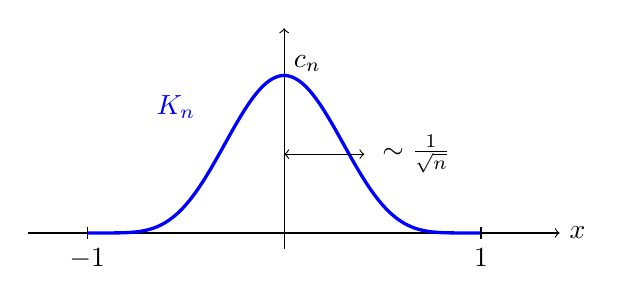
\begin{tikzpicture}[xscale=2.5, yscale=1]
  \draw[->] (-1.3,0) -- (1.4,0) node[right] {$x$};
  \draw[->] (0,-0.2) -- (0,2.6);
  \draw[blue, very thick, domain=-1:1, samples=120, smooth] plot (\x, {2*(1-\x*\x)^6});
  \draw (-1,0.08) -- (-1,-0.08) node[below] {$-1$};
  \draw (1,0.08) -- (1,-0.08) node[below] {$1$};
  \node[right] at (0,2.15) {$c_n$};
  \draw[<->] (0,1.0) -- (0.408,1.0);
  \node[right] at (0.45,1.0) {$\sim\frac{1}{\sqrt n}$};
  \node[blue] at (-0.55,1.6) {$K_n$};
\end{tikzpicture}
